%%%%%%%%%%%%%%%%%%%%%%%%%%%%%%%%%%%%%%%%%%%%%%%%%%%%%%%%%%%%%%%%%%%%%%
% Lớp 10 | Đại số tổ hợp | Quy tắc cộng-quy tắc nhân
% Dạng 0D8?1-3: Bài toán kết hợp quy tắc cộng và quy tắc nhân
% Số câu: 26  (sinh tự động bởi tach_cau.py; từ nay thầy sửa trực tiếp file này)
%%%%%%%%%%%%%%%%%%%%%%%%%%%%%%%%%%%%%%%%%%%%%%%%%%%%%%%%%%%%%%%%%%%%%%

%%%%%%%%%%%%%%%% TRẮC NGHIỆM 4 PHƯƠNG ÁN %%%%%%%%%%%%%%%%

% nguồn: MaHoaNH_TracNghiem_Lop10
\begin{ex}%[0D8N1-3]%[ma:b3020f8a]
	Một người có $5$ cái áo khác nhau trong đó $3$ áo màu trắng và $2$ áo màu xanh, có $3$ cái cà vạt khác nhau trong đó có $1$ cà vạt màu đỏ và $2$ cà vạt màu vàng. Hỏi người đó có bao nhiêu cách phối một bộ đồ  biết nếu chọn áo xanh thì không cà vạt màu đỏ.
	 \choice
		 {\True $15$}
		 {$5$}
		 {$10$}
		{$13$} 
	\loigiai{ 
		\begin{enumerate}[TH1:]
			\item Chọn áo  màu trắng có $3$ cách.\\
			Chọn cà vạt có  $3$ cách\\
			 Vậy có $3\cdot3=9$ cách phối một bộ đồ.
			\item Chọn áo  màu xanh có $2$ cách.\\
			Chọn cà vạt  màu vàng có $3$ cách.\\
			Vậy có  $3\cdot2=6$ cách phối một bộ đồ.
		\end{enumerate}
		 Theo qui tắc cộng ta có cách phối một bộ đồ thỏa mãn yêu cầu là $6+9=15$ cách.
	 }
\end{ex}

% nguồn: MaHoaNH_TracNghiem_Lop10
\begin{ex}%[0D8H1-3]%[ma:80d6af0d]
	Có $3$ nam và $3$ nữ  cần xếp ngồi vào một hàng ghế. Hỏi có mấy cách xếp sao cho nam, nữ ngồi xen kẽ?
	 \choice
		{\True $72$} 
		{$74$} 
		 {$76$}
		{$78$} 
	 \loigiai{
		 Giả sử, ta đánh số các ghế lần lượt từ $1$ đến $6$.\\
		Đầu tiên, ta xếp $3$ bạn nam vào các ghế mang số chẵn, ta có $3!$ cách. Sau đó,  ta xếp $3$ bạn nữ vào các ghế số lẻ, ta có $3!$ cách. Vậy số cách xếp là $3!\cdot 3!=36$ cách.\\
		Trường hợp xếp $3$ bạn nam vào các ghế số lẻ, ta cũng  được kết quả tương tự trường hợp xếp nam vào ghế chẵn.\\
		Vậy số cách xếp  thỏa mãn bài toán là $36\cdot 2=72$ cách.
	} 
\end{ex}

% nguồn: MaHoaNH_TracNghiem_Lop10
\begin{ex}%[0D8H1-3]%[ma:0d13ca9f]
	 Trên giá sách có $10$ quyển sách Toán khác nhau, $8$ quyển sách Tiếng Anh khác nhau và $6$ quyển sách Lý khác nhau. Hỏi có bao nhiêu cách chọn hai quyển sách không cùng thuộc một môn?
	 \choice
		{$480$} 
		{$80$} 
		{$60$} 
		 {\True $188$}
	\loigiai{ 
		Số cách chọn $2$  quyển sách khác nhau gồm $1$ Toán và $1$ Tiếng Anh là $10\cdot8=80$.\\
		 Số cách chọn $2$ quyển sách khác nhau gồm $1$ Toán và $1$ Lý là $10\cdot6=60$.\\
		Số cách chọn $2$ quyển sách khác nhau gồm $1$ Tiếng Anh và $1$ Lý là  $8\cdot6=48$.\\
		Theo  quy tắc cộng, số cách chọn thỏa yêu cầu bài toán là $80+60+48=188$ cách.
	} 
\end{ex}

% nguồn: MaHoaNH_TracNghiem_Lop10
\begin{ex}%[0D8H1-3]%[ma:4599f496]
	Có bao nhiêu cách sắp xếp $3$ nữ  sinh, $3$ nam sinh thành một hàng dọc sao cho các bạn nam và nữ ngồi xen kẽ?
	\choice 
		{$6$} 
		{\True $72$} 
		{$720$} 
		{$144$} 
	 \loigiai{
		Giả sử, ta đánh số các  vị trí trên hàng dọc từ trên xuống dưới lần lượt từ $1$ đến $6$.\\
		Đầu tiên, ta xếp $3$ bạn nam vào các vị trí số chẵn, ta có $3!$ cách. Sau đó, ta xếp $3$ bạn nữ vào các vị trí số  lẻ, ta có $3!$ cách. Vậy số cách xếp là $3!\cdot 3!=36$ cách.\\
		Trường hợp xếp $3$ bạn nam vào các vị trí số lẻ, ta cũng được  kết quả tương tự trường hợp xếp nam vào vị trí số chẵn.\\
		Vậy số  cách xếp thỏa mãn bài toán là $36\cdot 2=72$ cách.
	 }
\end{ex}

% nguồn: MaHoaNH_TracNghiem_Lop10
\begin{ex}%[0D8H1-3]%[ma:8a28ff27]
	Một nhóm công nhân gồm $15$ nam và $5$ nữ. Người ta muốn chọn từ nhóm ra $5$ người để lập  thành một tổ công tác gồm $1$ tổ trưởng là nam, $1$ tổ phó là nam và ba người còn lại có ít nhất $1$ nữ. Hỏi có bao nhiêu cách lập tổ công tác?
	\choice 
		 {\True $111300$}
		 {$233355$}
		{$109200$} 
		{$112342$} 
	 \loigiai{
		Số cách  chọn $1$ tổ trường nam là $15$.\\
		 Số cách chọn $1$ tổ phó nam là $14$.\\
		Số cách chọn ba người còn lại  là $5\cdot \mathrm{C}^2_{13}+\mathrm{C}^2_{5}\cdot 13+\mathrm{C}^3_{5}=530$.\\
		 Vậy có $15\cdot 14\cdot 530=111300$ cách.
	 }
\end{ex}

% nguồn: MaHoaNH_TracNghiem_Lop10
\begin{ex}%[0D8H1-3]%[ma:f4a919e3]
	Cho hai đường thẳng song song $d$ và $d'$. Trên đường thẳng $d$ lấy $5$ điểm khác nhau, trên đường thẳng $d'$ lấy $8$ điểm khác nhau. Hỏi có thể vẽ được bao nhiêu vectơ mà các điểm đầu và điểm cuối  không cùng nằm trên một đường thẳng.
	 \choice
		{$32$} 
		 {$13$}
		 {\True $80$}
		{$40$} 
	\loigiai{ 
		\begin{itemize}
			\item Chọn điểm đầu trên $d_1$ và điểm  cuối trên $d_2$ thì số vectơ có được là $5\cdot8=40$.
			\item Chọn điểm đầu trên $d_2$ và  điểm cuối trên $d_1$ thì số vectơ có được là $5\cdot8=40$.
		\end{itemize}
		Vậy  số vectơ có được là $40+40=80$.
	} 
\end{ex}

% nguồn: MaHoaNH_TracNghiem_Lop10
\begin{ex}%[0D8H1-3]%[ma:e71f00ce]
	Từ tập $X=\left\{0,1,2,3,4,5\right\}$ chọn ra số các số chia hết cho $5$ có $3$ chữ số khác nhau. Số  các số này là
	\choice 
		{\True  $36$}
		 {$40$}
		{$32$} 
		{$320$} 
	 \loigiai{
		Gọi số cần tìm có dạng $\overline{a_1  a_2 a_3}$.\\
		Nếu $a_3=5$ thì $a_1$ có  $4$ cách chọn;
		 $a_2$ có $4$ cách chọn.\\
		Nếu $a_3=0$ thì $a_1$ có $5$ cách  chọn; $a_2$ có $4$ cách chọn.\\
		Vậy có $16+20=36$ số. 
	} 
\end{ex}

% nguồn: MaHoaNH_TracNghiem_Lop10
\begin{ex}%[0D8H1-3]%[ma:ec38798d]
	Từ các chữ số $1$, $2$, $3$, $4$, $5$, $6$  có thể lập được bao nhiêu số tự nhiên bé hơn $100$?
	\choice 
		 {$36$}
		 {$62$}
		{$54$} 
		{\True $42$} 
	 \loigiai{
		Các số  bé hơn $100$ chính là các số có một chữ số và hai chữ số được hình thành từ tập $A=\left\{1,2,3,4,5,6\right\}$.
		\begin{itemize}
			\item Từ tập $A$ có  thể lập được $6$ số có một chữ số.
			\item Gọi số  có hai chữ số có dạng $\overline{ab}$ với $(a, b)\in A$.\\
			Trong  đó
			\begin{itemize}
				\item $a$ được chọn từ tập $A$  (có $6$ phần tử) nên có $6$ cách chọn.
				\item $b$ được chọn từ tập $A$ (có $6$ phần tử) nên có $6$ cách chọn. 
			\end{itemize}
			 Như vậy, ta có $6\cdot 6=36$ số có hai chữ số.
		\end{itemize}
		Vậy từ $A$  có thể lập được $36+6=42$ số tự nhiêu bé hơn $100$.
	 }
\end{ex}

% nguồn: MaHoaNH_TracNghiem_Lop10
\begin{ex}%[0D8H1-3]%[ma:0d8a4e35]
	Tô màu các cạnh của hình vuông $ABCD$ bởi $6$ màu khác nhau sao cho mỗi cạnh được tô bởi một màu và hai cạnh kề nhau thì tô bởi hai màu khác nhau. Hỏi có bao nhiêu  cách tô?
	 \choice
		 {$360$}
		{$480$} 
		{$600$} 
		{\True $630$} 
	\loigiai{ 
		\textbf{Trường hợp 1:} Tô cạnh $AB$ và $CD$ khác  màu:\\
		Số cách tô cạnh $AB$: $6$ cách.\\ 
		Số cách tô cạnh  $BC$: $5$ cách.\\
		Số cách  tô cạnh $CD$: $4$ cách.\\
		Số cách  tô cạnh $AD$: $4$ cách.\\
		Theo quy  tắc nhân ta có: $6\cdot5\cdot4\cdot4=480$ cách tô cạnh $AB$ và $CD$ khác màu.\\
		\textbf{Trường hợp 2:} Tô cạnh $AB$  và $CD$ cùng màu:\\
		Số cách tô  cạnh $AB$: $6$ cách.\\
		Số cách tô cạnh $BC$: $5$ cách.\\ 
		Số cách tô cạnh $CD$: $1$ cách.\\ 
		Số cách  tô cạnh $AD$: $5$ cách.\\
		 Theo quy tắc nhân ta có: $6\cdot5\cdot1\cdot5=150$ cách tô cạnh $AB$ và $CD$ cùng màu.
		Vậy số cách  tô màu thỏa đề bài là: $480+150=630$ cách.
	} 
\end{ex}

% nguồn: MaHoaNH_TracNghiem_Lop10
\begin{ex}%[0D8H1-3]%[ma:eb26d654]
	Từ các chữ số $0$, $1$, $2$, $3$, $4$, $5$ có thể lập được bao nhiêu  chữ số chẵn gồm $4$ chữ số khác nhau?
	 \choice
		{\True $156$} 
		{$144$} 
		 {$96$}
		 {$134$}
	 \loigiai{
		Gọi số cần tìm có dạng $\overline{abcd}$ với $\left\{a, b, c, d\right\}\in A=\left\{0,1, 2,3,  4,5\right\}$.\\
		Vì $\overline{abcd}$ là số chẵn $\Rightarrow d\in \left\{0,2, 4\right\}$. 
		\begin{itemize}
			\item  Trường hợp $1$. \\
			Nếu $d=0$, số cần tìm là $\overline{abc0}$.\\Khi đó\\ 
			$a$ được chọn từ tập $A\setminus\{0\}$ nên có  $5$ cách chọn.\\
			$b$ được chọn từ tập $A\setminus\left\{0, a\right\}$  nên có $4$ cách chọn.\\
			$c$ được chọn từ tập $A\setminus\left\{0, a,  b\right\}$ nên có $3$ cách chọn.\\
			Như vậy có tất cả $5\cdot 4\cdot 3=60$ số có  dạng $\overline{abc0}$.
			 \item Trường hợp $2$.\\
			Nếu $d\in\left\{2;  4\right\}\Rightarrow d$ có $2$ cách chọn.\\
			 Khi đó\\
			$a$ có $4$ cách chọn(khác $0$ và $d$),\\ $b$ có $4$ cách chọn và $c$ có $3$ cách chọn.\\ 
			Như vậy có tất cả $2\cdot 4\cdot 4\cdot 3=96$ số  cần tìm như trên.
		\end{itemize}
		Vậy có tất cả $60+96=156$ số cần  tìm.
	 }
\end{ex}


%%%%%%%%%%%%%%%% ĐÚNG/SAI %%%%%%%%%%%%%%%%

% nguồn: MaHoaNH_DungSai_Lop10
\begin{ex}%[0D8N1-3]%[ma:ad26d541]
	Một hộp đựng $3$ viên bi đỏ, $4$ viên bi vàng  và $5$ viên bi xanh.
	 \choiceTF
		{\True Có $47$ cách  chọn hai viên bi khác màu}
		{Có $12$  cách chọn hai viên bi khác màu}
		{\True Có $12$ cách  chọn một viên bi}
		{\True Có $60$ cách chọn ba viên bi khác  nhau về màu}
	\loigiai{ 
		Chọn hai viên bi khác màu ta có các trường hợp: hai viên đỏ vàng, hai viên đỏ xanh hoặc hai viên vàng xanh.  Vậy có $3\cdot 4+3\cdot 5+4\cdot 5=47$ cách chọn hai viên bi khác màu.\\
		Có $3+4+5=12$ cách chọn một viên  bi.\\
		Chọn ba viên bi khác nhau về màu ta  cần một viên đỏ, một viên vàng và một viên xanh. Do đó, có $3\cdot 4\cdot 5=60$ cách chọn ba viên bi khác nhau về màu.
	 }
\end{ex}

% nguồn: MaHoaNH_DungSai_Lop10
\begin{ex}%[0D8N1-3]%[ma:1b9d4a4d]
	Một túi có $20$ viên bi khác nhau trong  đó có $7$ bi đỏ, $8$ bi xanh và $5$ bi vàng. Khi đó, xét tính \textbf{đúng}, \textbf{sai} của các mệnh đề sau
	 \choiceTF
		{\True Số cách chọn ba bi khác màu là $280$ cách} 
		{Số cách chọn hai viên khác màu, trong đó có  $1$ bi đỏ và $1$ bi vàng là $40$ cách}
		{\True Số cách chọn hai viên khác màu, trong đó có $1$ bi đỏ và $1$ bi xanh  là $56$ cách}
		{Số cách  chọn hai bi khác màu là $96$ cách}
	 \loigiai{
		\begin{itemchoice}
			\itemch \textbf{Đúng}. 
			Việc chọn ba viên bi khác màu phải tiến hành ba giai đoạn liên  tiếp:
			\begin{enumerate}[label=Giai đoạn \arabic*:, font = \bfseries, leftmargin=*]
				\item Chọn  một viên bi đỏ có $7$ cách.
				\item Chọn một viên bi  xanh có $8$ cách.
				\item Chọn một viên bi vàng  có $5$ cách.
			\end{enumerate}
			Số cách chọn ba bi khác màu là $7\cdot 8\cdot 5=280$ cách. 
			 \itemch \textbf{Sai}.
			Hai viên khác màu là bi đỏ và bi vàng.  Ta có số cách chọn là $7\cdot 5=35$ cách.
			\itemch \textbf{Đúng}. 
			Hai viên khác màu  là bi đỏ và bi xanh.
			\begin{enumerate}[label=Giai đoạn \arabic*:, font = \bfseries, leftmargin=*]
				\item Chọn một viên bi đỏ có $7$ cách. 
				\item Chọn  một viên bi xanh có $8$ cách.
			\end{enumerate}
			Số cách chọn trường hợp này  là $7\cdot 8=56$ cách.
			\itemch  \textbf{Sai}.
			Hai viên khác màu là bi xanh và bi vàng. Ta  có số cách chọn là $8\cdot 5=40$ cách.\\
			Vậy số cách chọn  hai bi khác màu là $56+35+40=131$ cách.
		\end{itemchoice}
	 }
\end{ex}

% nguồn: MaHoaNH_DungSai_Lop10
\begin{ex}%[0D8N1-3]%[ma:5ae22fa6]
	Trên giá sách có $5$ quyển sách Tiếng Anh khác nhau, $6$ quyển sách Toán khác nhau và $8$ quyển sách Tiếng Việt  khác nhau. Xét tính đúng sai của các mệnh đề sau
	\choiceTF 
		{\True Số cách chọn ba quyển sách khác môn  là $240$ cách}
		{Số cách chọn hai quyển gồm Tiếng Anh và Toán  là $11$ cách}
		{\True Số cách chọn ra một quyển sách từ số sách đã  cho là $19$ cách}
		{\True Số cách chọn hai quyển sách khác môn  là $118$ cách}
	 \loigiai{
		\begin{itemchoice}
			 \itemch \textbf{Đúng}.
			\begin{itemize}
				\item Chọn một quyển sách Tiếng Anh có $5$  cách.
				 \item Chọn một quyển sách Toán có $6$ cách.
				\item Chọn một quyển  sách Tiếng Việt có $8$ cách.
			\end{itemize}
			 Số cách chọn ba quyển sách khác môn là $5\cdot6\cdot 8=240$ cách.
			 \itemch \textbf{Sai}. Chọn được hai quyển gồm Tiếng Anh và Toán.\\
			 Số cách chọn là $5\cdot 6=30$ cách.
			\itemch  \textbf{Đúng}.
			Số cách chọn ra một quyển sách  từ số sách đã cho $5+6+8=19$ cách.
			 \itemch \textbf{Đúng}.
			\begin{enumerate}[TH1:]
				\item Chọn được hai quyển gồm  Tiếng Anh và Toán.\\
				Số  cách chọn là $5\cdot6=30$ cách.
				\item Chọn được hai quyển gồm  Tiếng Anh và Tiếng Việt.\\
				Số cách  chọn là $5\cdot 8=40$ cách.
				\item  Chọn được hai quyển gồm Toán và Tiếng Việt.\\
				 Số cách chọn là $6\cdot 8=48$ cách.
			\end{enumerate}
			Số cách chọn hai  quyển sách khác môn là $30+40+48=118$ cách.
		\end{itemchoice}
	} 
\end{ex}

% nguồn: MaHoaNH_DungSai_Lop10
\begin{ex}%[0D8H1-3]%[ma:5cc2852f]
	Một câu lạc bộ hội họa có $7$ học sinh lớp $10$, $8$ học sinh lớp $11$, $9$ học sinh lớp $12$. Cần  chọn $2$ học sinh để đại diện câu lạc bộ đi thi một cuộc thi về vẽ phong cảnh.
	\choiceTF 
		{\True Có $56$ cách chọn hai học sinh gồm $1$  học sinh lớp $10$ và $1$ học sinh lớp $11$}
		{\True  Có $63$ cách chọn hai học sinh gồm $1$ học sinh lớp $10$ và $1$ học sinh lớp $12$}
		{\True Có $72$ cách chọn hai học sinh gồm $1$ học sinh lớp  $11$ và $1$ học sinh lớp $12$}
		 {Có $24$ cách chọn hai học sinh khác lớp}
	\loigiai{ 
		Có  $7\cdot 8=56$ cách chọn hai học sinh gồm $1$ học sinh lớp $10$ và $1$ học sinh lớp $11$.\\
		Có $7\cdot 9=63$ cách  chọn hai học sinh gồm $1$ học sinh lớp $10$ và $1$ học sinh lớp $12$.\\
		Có $8\cdot 9=72$ cách chọn hai học sinh gồm $1$ học sinh lớp  $11$ và $1$ học sinh lớp $12$.
	} 
\end{ex}

% nguồn: MaHoaNH_DungSai_Lop10
\begin{ex}%[0D8H1-3]%[ma:6eb57f1e]
	Trên một giá sách có $4$ quyển sách Toán, $5$ quyển sách Vật lí và $6$ quyển sách Hóa học. Các quyển sách đôi một khác nhau. 
	 \choiceTF
		{\True Có $15$ cách lấy một quyển  sách tùy ý từ giá sách}
		{\True Có $9$ cách lấy một quyển sách Toán hoặc Vật lý từ giá sách} 
		{Có $10$ cách lấy hai quyển sách  gồm Toán và Hóa học từ giá sách}
		{\True Có $120$ cách lấy ba quyển sách có đủ ba môn học từ giá sách} 
	 \loigiai{
		\begin{itemchoice}
			\itemch Trên  giá sách có $4+5+6=15$ quyển sách.\\
			Lấy $1$ quyển tùy ý từ $15$  quyển nên có $15$ cách lấy.
			\itemch Lấy một quyển sách Toán hoặc Vật lý từ giá sách.\\ 
			Lấy  một quyển Toán có $4$ cách lấy.\\
			 Lấy một quyển Vật lý có $5$ cách lấy.\\
			Việc lấy sách được hoàn thành bởi một trong hai hành động trên nên  theo quy tắc cộng có $4+5=9$ cách lấy.
			\itemch Lấy hai quyển sách gồm  Toán và Hóa học từ giá sách.\\
			Lấy  một quyển Toán có $4$ cách lấy.\\
			Lấy một quyển Hóa học  có $6$ cách lấy.\\
			Việc lấy sách được hoàn thành bởi liên tiếp hai hành động trên nên  theo quy tắc nhân có $4\cdot6=24$ cách lấy.
			\itemch Lấy ba quyển  sách có đủ ba môn học từ giá sách.\\
			Lấy  một quyển Toán có $4$ cách lấy.\\
			Lấy một  quyển Vật lý có 5 cách lấy.\\
			Lấy một quyển Hóa học  có 6 cách lấy.\\
			Việc lấy sách được hoàn thành bởi liên tiếp ba hành động trên nên theo quy tắc  nhân có $4\cdot5\cdot6=120$ cách lấy.
		\end{itemchoice}
	 }
\end{ex}

% nguồn: MaHoaNH_DungSai_Lop10
\begin{ex}%[0D8H1-3]%[ma:87a1670b]
	Các  thành phố $A$, $B$, $C$ được nối với nhau bởi các con đường như hình vẽ.
	\begin{center}
		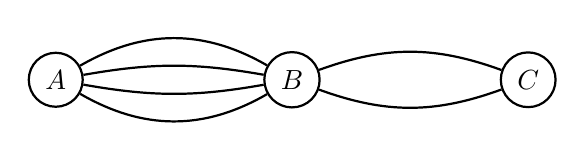
\begin{tikzpicture}[node distance={3cm},thick,main/.style = {draw,circle}]
				\node[main] (1)  {$A$};
				\node[main] (2) [right of=1]  {$B$};
				\node[main] (3) [right  of=2] {$C$};
				\draw (1)  to [out=30,in=150,looseness=1] (2);
				\draw (1) to [out=10,in=170,looseness=1] (2); 
				\draw (1) to  [out=-10,in=-170,looseness=1] (2);
				\draw  (1) to [out=-30,in=-150,looseness=1] (2);
				 \draw (2) to [out=20,in=160,looseness=1] (3);
				\draw  (2) to [out=-20,in=-160,looseness=1] (3);
			\end{tikzpicture}
	\end{center}
	 \choiceTF
		{\True  Có $2$ cách đi từ thành phố $C$ đến thành phố $B$}
		{\True Có tất cả $6$ con đường trong hình  vẽ}
		{Có $6$ cách đi từ  thành phố $A$ đến thành phố $C$ mà qua $B$ chỉ một lần}
		{Có $8$ cách đi xuất phát từ thành phố $B$  đến thành phố $A$ và quay ngược lại thành phố $B$}
	 \loigiai{
		\begin{itemchoice}
			\itemch Chỉ có $2$ con đường nối từ thành phố $C$ đến thành  phố $B$.
			\itemch Có $4$ con đường nối từ thành phố $A$  đến thành phố $B$.\\
			 Có $2$ con đường nối từ thành phố $B$ đến thành phố $C$.\\
			Do đó có tất cả $4+2=6$ con đường. 
			\itemch Có $4$  con đường nối từ thành phố $A$ đến thành phố $B$.
			Có $2$ con đường nối  từ thành phố $B$ đến thành phố $C$.\\
			Do đó số cách đi từ thành phố $A$ đến  thành phố $C$ là $4\cdot2=8$.
			\itemch Đi từ thành phố $A$ đến thành phố $B$ có $4$ cách và  ngược lại.
			Do  đó, số cách đi cần tìm là $4\cdot4=16$.
		\end{itemchoice}
	} 
\end{ex}

% nguồn: MaHoaNH_DungSai_Lop10
\begin{ex}%[0D8V1-3]%[ma:76a4bab6]
	 Cho các chữ số $0$, $1$, $2$, $3$, $4$, $5$.
	\choiceTF{\True Có $180$  số tự nhiên có $3$ chữ số được lập từ các chữ số đã cho}
		{\True Có $100$ số tự  nhiên có $3$ chữ số đôi một khác nhau được lập từ các chữ số đã cho}
		{Có $93$ số tự nhiên lẻ có $3$ chữ số được lập  từ các chữ số đã cho}
		{Có $155$ số tự nhiên chẵn có $3$ chữ số đôi một khác nhau  được lập từ các chữ số đã cho}
	\loigiai{Gọi số cần tìm có dạng $\overline{abc}$ với $a,b,c\in\{0;1;2;3;4;5\}$  và $a\ne 0$.
		\begin{itemchoice}
			\itemch 
			 $a$ có $5$ cách chọn, $b$ có $6$ cách chọn, $c$ có $6$ cách chọn.\\
			Vậy có $5\cdot 6 \cdot  6=180$ số thỏa yêu cầu bài toán.
			\itemch $a$ có $5$ cách chọn, $b$ có $5$ cách chọn,  $c$ có $4$ cách chọn.\\
			Vậy có $5\cdot 5 \cdot 4=100$ số thỏa yêu cầu  bài toán.
			\itemch $a$ có $5$ cách chọn, $b$ có $6$ cách chọn, $c$ có $3$ cách  chọn.\\
			Vậy có $5\cdot  6 \cdot 3=90$ số thỏa yêu cầu bài toán.
			\itemch Xét các trường hợp  sau
			\begin{itemize}
				\item Trường hợp 1. $c=0$, ta có\\ 
				chọn chữ số $c$ có  1 cách.\\
				chọn và sắp xếp $2$ chữ số $a$, $b$  có $\mathrm{A}_5^2$ cách.\\
				Do đó, có $1 \cdot \mathrm{A}_5^2= 20$  (số).
				\item Trường hợp 2. $c\in \{2; 4\}$, ta có\\ 
				chọn chữ số  $c$ có $2$ cách.\\
				chọn chữ  số $a$ có $4$ cách.\\
				chọn  chữ số $b$ có $4$ cách.\\
				Do đó, có $2\cdot  4 \cdot 4= 32$ (số).
			\end{itemize}
			Vậy theo quy tắc cộng, số các số thoả mãn bài toán là $20+32=  52$ (số).
		\end{itemchoice}
	} 
\end{ex}

% nguồn: MaHoaNH_DungSai_Lop10
\begin{ex}%[0D8V1-3]%[ma:3e4a4f0c]
	Lập các số tự nhiên có $4$ chữ số  từ các chữ số $1$; $2$; $3$; $4$; $5$; $6$.
	\choiceTF 
		{\True Có $648$ số  chẵn}
		 {\True Có $648$ số lẻ}
		{\True Có $120$ số lẻ có các chữ số khác nhau đôi một và chữ số hàng  trăm lớn hơn $2$}
		{Có $48$ số  lẻ có các chữ số khác nhau đôi một và chữ số hàng trăm chẵn đồng thời lớn hơn $2$}
	\loigiai{ 
	\begin{itemchoice}
		\itemch 
		 Gọi số có $4$ chữ số có dạng $\overline{abcd}$.\\
		Chọn số cho $a$, $b$, $c$  có $6^3$ cách.\\
		Chọn số chẵn cho  $d$ có $3$ cách.\\
		Vậy số cách là  $6^3\cdot3=648$.
		 \itemch
		Gọi số có $4$ chữ số có dạng  $\overline{abcd}$.\\
		Chọn số cho $a$,  $b$, $c$ có $6^3$ cách.\\
		Chọn số lẻ cho $d$ có  $3$ cách.\\
		 Vậy số cách là $6^3\cdot3=648$.
		\itemch 
		Gọi số có $4$ chữ  số có dạng $\overline{abcd}$.\\
		Ta  xét $2$ trường hợp \\
		\textbf{Trường hợp 1.} $d=1$.\\ 
		 Chọn $b>2$ có $4$ cách.\\
		Chọn $c$ có $4$  cách.\\
		Chọn $a$ có $3$ cách. \\ 
		\textbf{Trường hợp 2.} $d\in \{3;5\}$ có $2$ cách.\\ 
		Chọn $b>2$ có $3$  cách.\\
		Chọn $c$ có $4$  cách.\\
		Chọn $a$  có $3$ cách. \\
		Vậy tổng  số cách là $4\cdot 4\cdot 3+2\cdot 3\cdot 4\cdot 3=120$ cách.
		\itemch Gọi số có $4$  chữ số có dạng $\overline{abcd}$.\\
		Chọn số cho $d$  có $3$ cách.\\
		Chọn số cho $b$ có $2$ cách.\\ 
		Chọn số cho $c$ có $4$  cách.\\
		Chọn số cho $a$ có  $3$ cách.\\
		Vậy tổng số cách là $3\cdot  2\cdot 4\cdot 3=72$.
	\end{itemchoice}
	} 
\end{ex}


%%%%%%%%%%%%%%%% TRẢ LỜI NGẮN %%%%%%%%%%%%%%%%

% nguồn: MaHoaNH_TraLoiNgan_Lop10
\begin{bt}%[0D8H1-3]%[ma:5d85890f]
	Một trường THPT  được cử một học sinh đi dự trại hè toàn quốc. Nhà trường quyết định chọn một học sinh giỏi lớp 11A hoặc lớp 12A. Hỏi nhà trường có bao nhiêu cách chọn, nếu biết rằng lớp 11A có $20$ học sinh giỏi và lớp 12A có $22$ học sinh giỏi?
	\shortans{42} 
	 \loigiai{
		Nhà trường có hai  phương án để thực hiện là
		\begin{enumerate}[TH 1:]
			\item Chọn một học sinh  giỏi từ lớp 11A có $20$ cách.
			\item Chọn  một học sinh giỏi từ lớp 12A có $22$ cách.
		\end{enumerate}
		Theo quy tắc cộng, nhà trường sẽ  có $20+22=42$ cách chọn thỏa mãn.
	 }
\end{bt}

% nguồn: MaHoaNH_TraLoiNgan_Lop10
\begin{bt}%[0D8V1-3]%[ma:25405452]
	Mật khẩu của một trang web là một dãy có từ $2$ tới $3$ kí tự, trong đó kí tự đầu tiên là một trong $26$ chữ cái inthường trong bảng chữ cái tiếng Anh (từ a đến z), mỗi kí tự còn lại là một chữ số từ $0$ đến $9$. Hỏi có thể tạo được bao nhiêu mật  khẩu khác nhau?
	 \shortans{2860}
	\loigiai{ 
		Xét  các trường hợp sau
		\begin{itemize}
			\item Trường hợp 1. Mật  khẩu gồm 2 kí tự.\\
			Chọn kí  tự đầu tiên, có $26$ cách.\\
			Chọn kí tự thứ hai, có $10$ cách.\\ 
			Theo quy tắc nhân, có $26 \cdot 10=  260$ cách.
			\item  Trường hợp 2. Mật khẩu gồm 3 kí tự.\\
			Chọn kí tự đầu tiên, có  $26$ cách.\\
			Chọn 2 kí tự tiếp  theo, có $10^2$ cách.\\
			Theo quy tắc  nhân, có $26 \cdot 10^2= 2600$ cách.
		\end{itemize}
		Vậy theo quy tắc cộng, số  cách tạo mật khẩu thoả mãn bài toán là $260+2600= 2860$ cách.
	 }
\end{bt}


%%%%%%%%%%%%%%%% TỰ LUẬN %%%%%%%%%%%%%%%%

% nguồn: MaHoaNH_TuLuan_Lop10
\begin{bt}%[0D8H1-3]%[ma:cd50f8e5]
	Cho tập $X=\{0; 1; 2; 3; 4; 5; 6; 7; 8; 9\}$. Hỏi  có bao nhiêu số tự nhiên có $5$ chữ số khác nhau từ $X$ và là số chẵn?
	\loigiai{ 
		Gọi $\overline{abcde}$ là số tự  nhiên có $5$ chữ số khác nhau từ $X$ và là số chẵn.
		\begin{itemize}
			\item Xét trường  hợp $e=0$.\\
			Chọn $a \neq 0$  (tức là $a$ cũng khác $e$) có $9$ cách chọn.\\
			Mỗi chữ số $b$, $c$, $d$ lần lượt có $8$, $7$, $6$ cách chọn. Khi đó,  ta có được $1\cdot9\cdot8\cdot7\cdot6=3\,024$ số.
			\item Xét trường hợp $e\in\left\{2;  4; 6; 8\right\}$. Chọn $e$ có $4$ cách chọn.\\
			Chọn $a$ với $a\neq 0$, $a\neq e$,  ta có $8$ cách chọn.\\
			Mỗi chữ số $b$, $c$, $d$ lần lượt có $8$,  $7$, $6$ cách chọn. Khi đó ta có được $4\cdot8\cdot8\cdot7\cdot6=10\,752$ số.\\
			Vậy số các số tự  nhiên thỏa mãn $3\,024+10\,752=13\,776$ số.
		\end{itemize}
	 }
\end{bt}

% nguồn: MaHoaNH_TuLuan_Lop10
\begin{bt}%[0D8V1-3]%[ma:43b2b1e9]
	Từ các chữ số $0$, $1$, $2$, $3$, $4$, $5$, $6$, $7$, $8$ có thể  lập được bao nhiêu số tự nhiên chẵn có $4$ chữ số khác nhau đôi một và không lớn hơn $4\,568$?
	 \loigiai{
		Gọi số cần tìm có dạng $\overline{a b c d}$. Xảy  ra các trường hợp sau
		\begin{enumerate}[label=Trường hợp \arabic*:, font = \bfseries, leftmargin=*]
			\item $a<4$. Chọn  $a\in\left\{1,2,3\right\}$ xảy ra hai tình huống:
			\begin{itemize}
				\item $a\in\left\{1,3\right\}$. Chọn $a$ có $2$ cách. Chọn $d\in\{0,2,4,6,8\}$ có $5$ cách. Chọn $b\neq a,  d$ có $7$ cách. Chọn $c\neq a, b, d$ có $6$ cách.
				\item $a=2$. Chọn $d\in\{0,4,6,8\}$ có $4$ cách. Chọn $b\neq a, d$ có $ 7$ cách. Chọn  $c\neq a, b, d$ có $6$ cách.
			\end{itemize}
			Vậy số kết quả  trong trường hợp này là $2\cdot 5\cdot7 \cdot6+4\cdot7 \cdot6=588$ số.
			 \item $a=4, b<5$. Chọn $b\in\{0,1,2,3\}$ xảy ra hai tình huống:
			\begin{itemize}
				\item $b\in\{1,3\}$.  Chọn $b$ có $2$ cách. Chọn $d\in\{0,2,6,8\}$ có $4$ cách. Chọn $c\neq a, b, d$ có $6$ cách.
				\item $b\in\{0,2\}$. Chọn $b$ có $2$ cách. Chọn $d\in\left\{0,2,6,8\right\}\setminus \left\{b\right\}$  có $3$ cách. Chọn $c\neq a, b, d$ có $6$ cách.
			\end{itemize}
			Vậy số kết quả trong trường hợp  này là $2\cdot 4\cdot6+2\cdot3 \cdot6=84$ số.
			\item $a=4, b=5, c<6$. Chọn $c\in\left\{0,1,2,3\right\}$ xảy ra hai tình huống:\\ 
			$c\in\{1,3\}$. Chọn $c$  có $2$ cách. Chọn $d\in\{0,2,6,8\}$ có $4$ cách.\\
			$c\in\{0,2\}$. Chọn $c$ có $2$ cách. Chọn $d\in\left\{0,2,6,8\right\}\setminus  \left\{b\right\}$ có $3$ cách.\\
			Vậy số kết  quả trong trường hợp này là $2\cdot4+2\cdot3=14$ số.
			\item $a=4$, $b=5$, $c=6$, $d\leq 8$. Chọn $d\in\left\{0{,}2{,}8\right\}$  có $3$ cách.\\
			Vậy số kết  quả trong trường hợp này là $3$ số.
		\end{enumerate}
	 Kết quả cần tìm là $588+84+14+3=689$ số.}
\end{bt}

% nguồn: MaHoaNH_TuLuan_Lop10
\begin{bt}%[0D8B1-3]%[ma:13d55ddf]
	Từ các chữ số $0$, $1$, $2$, $3$, $4$, $5$, $6$,  có thể lập được bao nhiêu số tự nhiên chẵn có $3$ chữ số đôi một khác nhau?
	\loigiai{ 
		Gọi số tự nhiên chẵn có $3$ chữ số đôi một  khác nhau là $n=\overline{abc}\,(a\ne b\ne c)$.
		\begin{itemize}
			\item  \textbf{Trường hợp 1:} $c=0$.\\
			Số cách chọn $a$,  $b$ là $\mathrm{A}_6^2=30$ cách.\\
			Do đó, ta  có $30$ số.
			\item \textbf{Trường hợp 2:} $c\in\{2;4;6\}$.\\ 
			 Chọn $c$ có $3$ cách.\\
			Chọn $a$  có $5$ cách ($a\ne0\ne c$).\\
			Chọn $b$ có $5$ cách ($b\ne a\ne c$).\\ 
			Theo quy tắc nhân, ta  có $3\cdot5\cdot5=75$ số.
		\end{itemize}
		Vậy số tự nhiên chẵn có $3$ chữ số đôi một khác nhau là  $n=30+75=105$ số.
	 }
\end{bt}

% nguồn: MaHoaNH_TuLuan_Lop10
\begin{bt}%[0D8B1-3]%[ma:9fc25bdf]
	Sử dụng 5 chữ số $0;1;2;3;4$ có thể lập được bao nhiêu số tự nhiên 
	\begin{enumerate}
		\item có  ba chữ số khác nhau?
		\item có 3 chữ số khác  nhau và bé hơn 300?
		 \item có các chữ số khác nhau và bé hơn 100?
	\end{enumerate}
	 \loigiai{
		\begin{enumerate}
			 \item Kí hiệu số có 3 chữ số khác nhau cần lập là $\overline{abc}$, trong đó $a, b, c$\ là các chữ số khác nhau từ các chữ số đã cho, $a \ne 0$. Đầu tiên, có 4 cách chọn chữ số $a$. Tiếp theo, có 4 cách chọn chữ số $b, 3$\ cách chọn chữ số $c$. Từ đó, có $4 \cdot 4 \cdot 3=48$ số tự nhiên thoả mãn yêu cầu.
			\item  Kí hiệu số $m$ như trên. Để $m<300$, điều kiện cần và đủ là $a<3$. Khi đó, có 2 cách chọn chữ số $a$ từ hai chữ số 1 và 2. Tiếp theo, có 4 cách chọn chữ số $b$, $3$ cách chọn chữ số $c$. Từ đó, có $2 \cdot 4 \cdot 3=24$ số tự nhiên thoả mãn yêu cầu.
			\item Kí hiệu $n$ là số tự nhiên lập được từ  các chữ số đã cho, $n<100$. Có 2 trường hợp như sau.\\
			Trường hợp 1: $n$ có một chũ số. Có 5 số như vậy từ 5 chữ số  đã cho.\\
			Trường hợp 2: $n$ có  hai chữ số, dạng $\overline{ab}$. Có 4 cách chọn chữ số $a, 4$\ cách chọn chữ số $b$. Từ đó, có $4 \cdot 4=16$ số $n$ như vậy.\\
			Áp dụng quy tắc cộng, có $5+16=21$ số tự nhiên  thoả mãn yêu cầu.
	\end{enumerate}}
\end{bt}

% nguồn: MaHoaNH_TuLuan_Lop10
\begin{bt}%[0D8Y1-3]%[ma:2f2945d5]
	 \immini{
	Trong một công viên, có các con đường nối bốn địa điểm $A, B, C$ và $D$ như Hình 2. Có bao nhiêu  cách chọn một đường đi từ $A$ đến $D$? Chỉ tính các đường đi qua mỗi địa điểm nhiều nhất một lần.
	}{ 
	\begin{tikzpicture}[line join=round,line cap=round,>=Stealth,thick,x=1cm,y=1cm,font=\footnotesize]
			\draw (0,0) coordinate (B) -- (0,1.5) coordinate (A) -- (2.5,1.5) coordinate  (C) to[out=-70,in=70] (2.5,0) coordinate (D)
				to[out=160,in=20]  (B)
				to[out=70,in=-70] (A) 
				to[out=-20,in=-160] (C) 
				to[out=-100,in=100]  (D)
				to[out=-160,in=-20]  (B)
				to[out=110,in=-110]  (A)
				to[out=20,in=160] (C) 
				 to[out=-50,in=50] (D)
				 (C) to[out=-130,in=130] (D);
			\foreach \i/\j in {A/135,B/-135,C/45,D/-45}{ 
				\fill[black] (\i) node[shift={(\j:6pt)}]{$\i$} circle (1pt); 
			 }
		\end{tikzpicture}
	} 
	\loigiai{ 
		Có  hai phương án để đi từ $A$ đến $D$.\\
		Phưong án 1: Đi từ $A$ qua $B$ rồi đến $D$. Có 3 cách chọn đường đi từ $A$ đến $B$, có 2 cách chọn đường  đi từ $B$ đến $D$. Theo quy tắc nhân, có $3 \cdot 2=6$ cách chọn đường đi từ $A$ qua $B$ rồi đến $D$.\\
		Phương án 2: Đi từ $A$ qua $C$ rồi đến $D$. Có 3 cách chọn đường đi từ $A$  đến $C$, có 4 cách chọn đường đi từ $C$ đến $D$. Theo quy tắc nhân, có $3 \cdot 4=12$ cách chọn đường đi từ $A$ qua $C$ rồi đến $D$.\\
	Áp dụng quy  tắc cộng, có $6+12=18$ cách chọn đường đi từ $A$ đến $D$.}
\end{bt}

% nguồn: MaHoaNH_TuLuan_Lop10
\begin{bt}%[0D8B1-3]%[ma:a651a683]
	\immini{ 
	Có  các con đường nối bốn ngôi làng A, B, C, D như trong hình bên. Có bao nhiêu cách chọn đường đi khác nhau
	\begin{enumerate}
		\item từ A qua B  rồi đến D?
		\item từ A đến D? Lưu  ý: Mỗi đường đi qua mỗi ngôi làng nhiều nhất một lần.
	\end{enumerate}
	 }{
	\begin{tikzpicture}[line join=round,line cap=round,>=Stealth,thick,x=1cm,y=1cm,font=\footnotesize]
			\draw  (0,0) coordinate (A) to[out=20,in=160] (4,0) coordinate (C)
				to[out=-70,in=70] (4,-2) coordinate  (D)
				to[out=-160,in=-20] (0,-2)  coordinate (B)
				 to[out=110,in=-110] (A)
				to[out=-20,in=-160] (C) 
				to[out=-110,in=110]  (D)
				 to[out=160,in=20] (B)
				to[out=70,in=-70] (A) 
				 to[out=-20,in=110] (D)
				 to[out=150,in=-60] (A);
			\foreach \i/\j  in {A/135,B/-135,C/45,D/-45}{
				\fill[black] (\i) node[shift={(\j:6pt)}]{$\i$} circle (1pt); 
			} 
		\end{tikzpicture}
	 }
	\loigiai{ 
		\begin{enumerate}
			 \item $2\cdot 2=4$.
			 \item $2\cdot 2+2\cdot 2+2=10$.
		\end{enumerate}
	} 
\end{bt}
